\FloatBarrier
\subsection{Question 4}
By changing the $cancel$ variable to $1$ in \autoref{code:str31}, we can get the system response when all zeros are cancelled out. 
\autoref{fig:str11} shows the system output and control effort for direct STR with zero cancellation.  \autoref{fig:str32} demonstrates the variation of parameter values over simulation time.

\begin{figure}
	\centering
	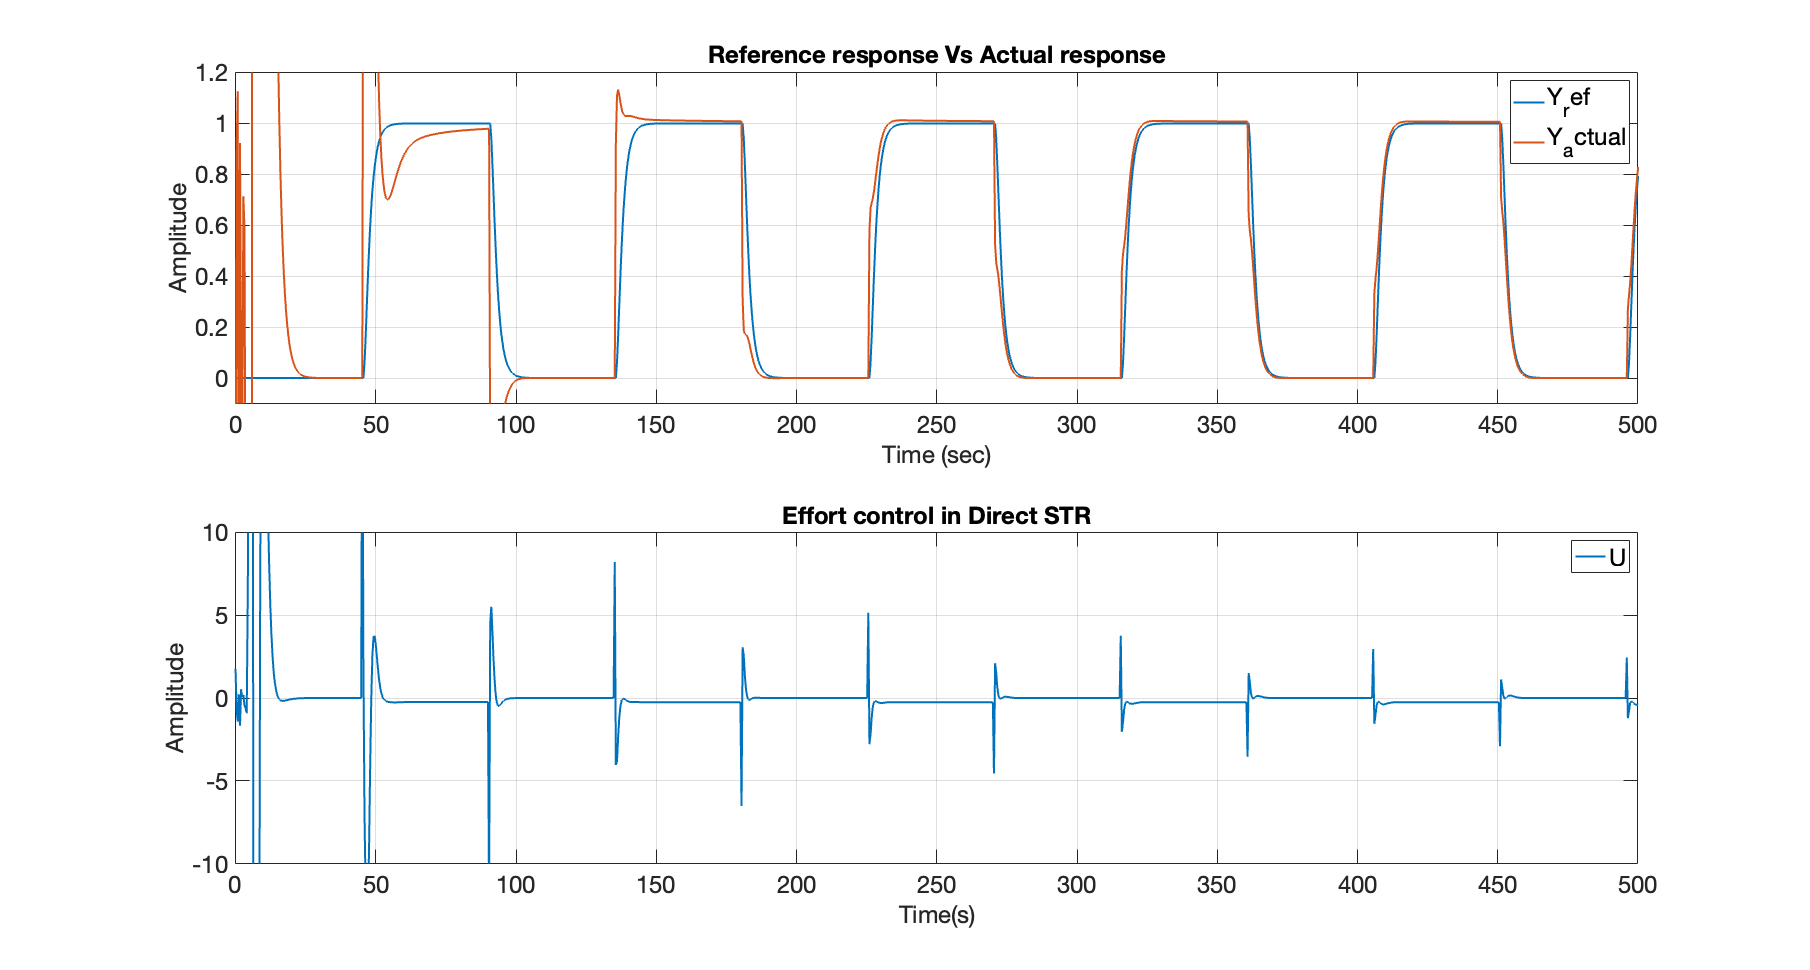
\includegraphics[width=\textwidth]{images/str41.png}
	\caption{direct STR ystem response with zero cancellation}
	\label{fig:str41}
\end{figure}

\begin{figure}
	\centering
	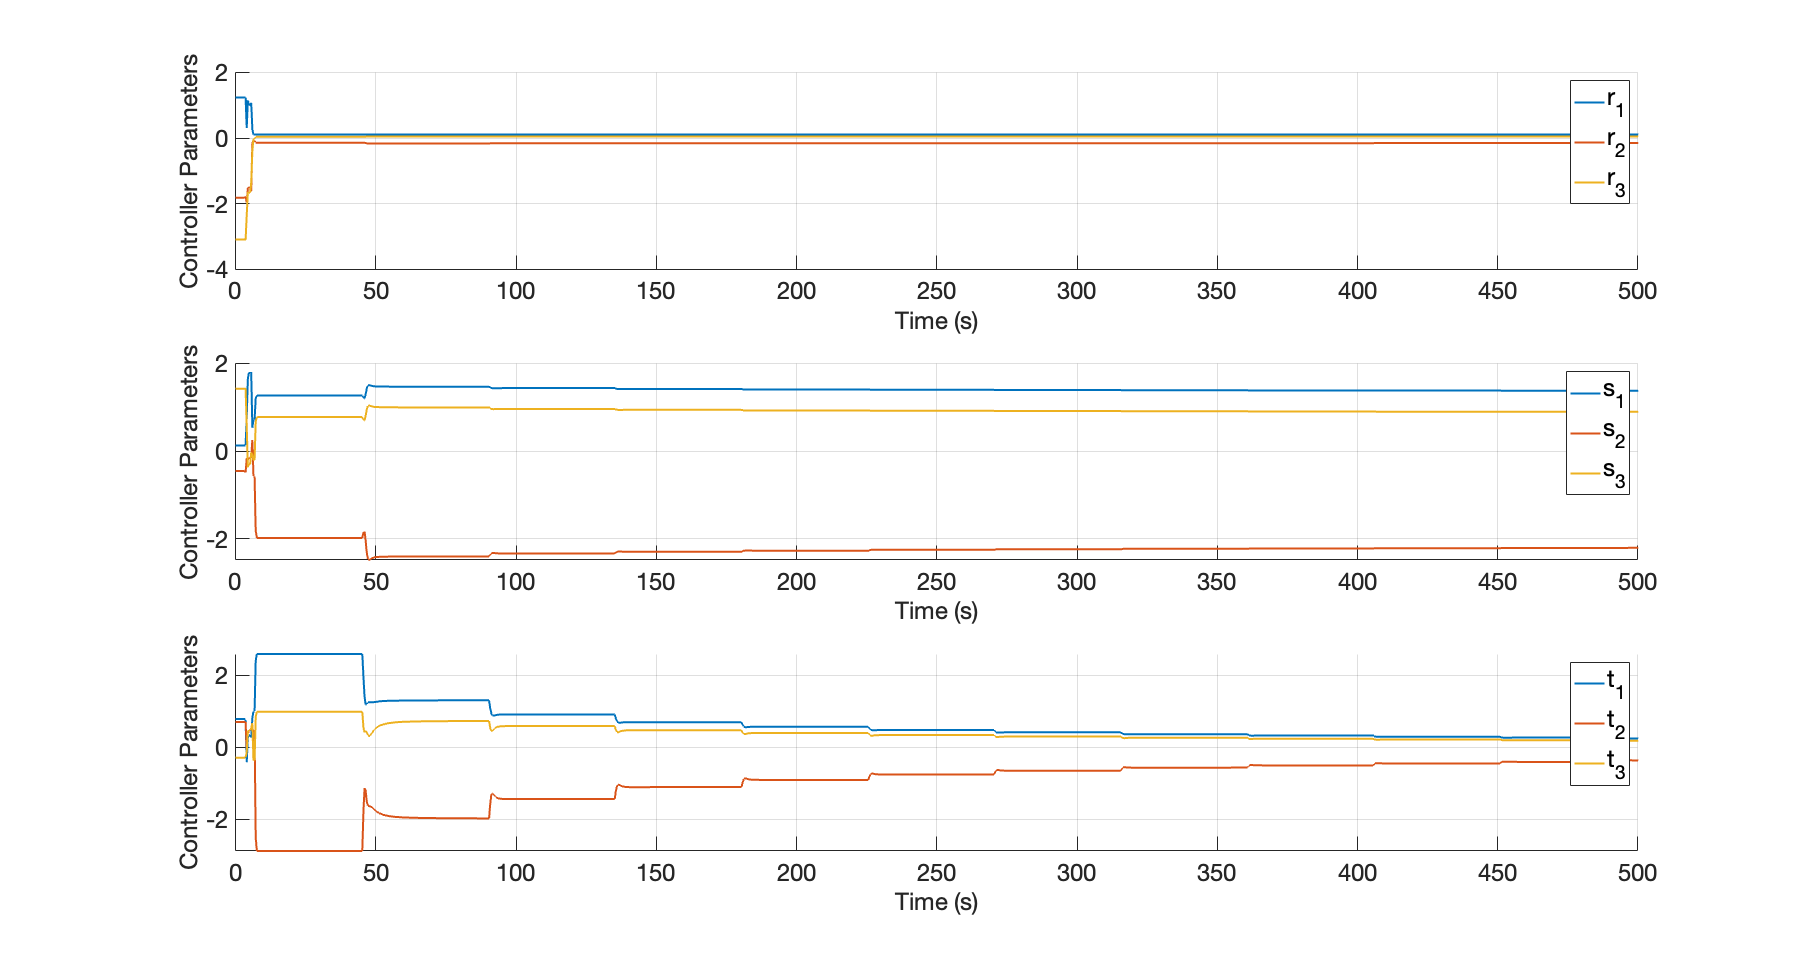
\includegraphics[width=\textwidth]{images/str42.png}
	\caption{System parameters in direct STR with zero cancellation}
	\label{fig:str42}
\end{figure}

The code  for this section is available at \lstinline|assignment2/part2/STR1_direct.m|. By changing the $change=0$ to $1$ system will determine values of  $R$ and $S$ and $T$ that are required for direct STR with zero cancellation. 


